\subsubsection{HTML (Weiland)}

HTML steht für "'Hypertext Markup Language"' und bezeichnet eine Auszeichnungssprache. HTML-Dateien werden hauptsächlich für Websites verwendet.


\paragraph{Aufbau}

Eine HTML-Datei ist grundsätzlich immer gleich aufgebaut. Sie besteht aus einem Header in dem unter anderem der Titel und die Meta-Daten bestimmt werden und einem Body in dem der eigentliche Inhalt, welcher angezeigt werden soll, steht.
\begin{lstlisting}[style=custom, language=HTML, caption={HTML-Tags}]
<!DOCTYPE html>
<html> 
	<head>
		/* Datei-Kopf */
	</head>
	<body>
		/* Inhalt der Datei */
	</body>
</html>
\end{lstlisting}

\paragraph{Elemente}
Jedes Element setzt sich aus einem Start-Tag und einem End-Tag zusammen. Im End-Tag wird nach der eckigen Klammer ein \enquote{/} geschrieben. (z.b. </html>).\\\\
Dies sind die wichtigsten Elemente, mit denen eine einfache Seite aufgebaut werden kann:
\begin{description}
\item[ ]
\begin{description} [style=nextline]
\item[<!DOCTYPE html>] Sollte zu Beginn jedes HTML-Dokuments stehen. Ist eigentlich kein richtiger HTML-Tag, wird jedoch benötigt um dem Browser den verwendeten Dokumenttyp mitzuteilen.
\item[<html>] Wird ganz zu Beginn, jedoch nach dem DOCTYPE-TAG,  eines Dokuments verwendet um das Dokument einzuleiten.
\item[<head>] Hier werden Informationen, wie Meta-DAten oder zum Beispiel der Titel hinterlegt.
\item[<body>] Leitet den Body, den Teil in dem die Ausgabe steht, ein.
\item[<title>] Dient dazu den Titel der Site, welcher unter anderem im Tab steht, anzugeben. Wenn kein Titel angegeben wird, wird stattdessen die URL verwendet.
\item[<script>] Mittels dieses Tags ist es möglich ein Script (z.B. JavaScript) in den HTML-Code einzubinden.
\item[<p>] Dieses Tag definiert einen Absatz. Es ist nicht möglich in einem Absatz ein anderes Blockelement, wie zum Beispiel eine Tabelle aufzurufen. Es ist grundsätzlich kein Endtag nötig, sollte aber dennoch gesetzt werden.
\item[<div>] Mittels dieses Tags wir ein Bereich definiert. Dies dient unter anderem dazu mittels CSS die Darstellung anzupassen. In einem Div darf nahezu jeder andere Tag verwendet werden, ausgenommen sind \enquote{<head>}, \enquote{<head>} und \enquote{<body>} 
\item[<hx>] Erzeugt eine Überschrift. Anstelle des X muss eine Zahl von 1 bis 6 eingefügt werden. Je nach Zahl ändert sich die Foramtierung des damit gekennzeichneten Texts.
\item[<a>] Hiermit wird ein Verweis erzeugt. Alles was zwischen dem Start- und dem End-Tag steht wird dann als Verweis gekennzeichnet. Zwischen diesen Tags können zum Beispiel auch Bilder stehen.
\item[<br />] Erzeugt einen Zeilenumbruch in der Ausgabe. \enquote{</br>} ist ebenso möglich, entspricht jedoch nicht dem XHTML-Standard.
\item[<img>] Bindet ein Bild in die Ausgabe ein. Die Quelle des Bildes muss mitgegeben werden. Zum Beispiel: \texttt{<img src="bild.png"}. Bei diesem Tag wird kein End-Tag benötigt.
\item[<table>] Mit diesem Tag wird eine Tabelle erzeugt. Standardmäßig besitzt eine Tabelle keine Umrandung, diese muss mittels \enquote{border} eingestellt werden
\begin{description}
\item[<tr>] In einer Tabelle muss jede Zeile mit diesem Tag gekennzeichnet werden.
\item[<th>] Erzeugt ein Tabellenüberschriftenfeld.
\item[<td>] Erzeugt ein normales Tabellenfeld.
\end{description}
\end{description}
\end{description}
\begin{lstlisting}[style=custom, language=HTML, caption={HTML-Tabelle}, label={lst:content_client_html_table}]
<!DOCTYPE html>
<html>
	<head>
		<title>Tabelle</title>
	</head>
	<body>
		<table border=1> 
			<tr>
				<th>Vorname</th>
				<th>Nachname</th>
				<th>Alter</th>
			</tr>
			<tr>
				<td>Franz</td>
				<td>Ose</td>
				<td>11</td>
			</tr>
			<tr>
				<td>Frank</td>
				<td>Furt</td>
				<td>22</td>
			</tr>
			<tr>
				<td>Ernst</td>
				<td>Gemeint</td>
				<td>33</td>
			</tr>
		<\table>
	</body>
</html>
\end{lstlisting}

\begin{figure}[H]
\centering
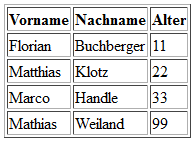
\includegraphics[keepaspectratio=true, width=5cm]{images/screenshots/html_table.png}
\caption{Mittels \autoref{lst:content_client_html_table} erzeugte Tabelle}
\label{fig:content_html_table}
\end{figure}

\paragraph{HTML5}
HTML5 ist die aktuellste Version von HTML. Die Entwicklung begann am 29. April 2009 und soll im Jahr 2014 fertiggestellt werden.\\ 
Mit der Einführung von HTML5 kommen viele neue Elemente, wie zum Beispiel \enquote{details} und \enquote{summary}, zum HTML-Standard dazu. Dies Elemente sind zum Teil interaktiv, was im bisherigen Standard nicht möglich war. So wird zum Beispiel mit dem Element \enquote{details} eine Ausgabe erzeugt die ein-oder ausgeklappt werden kann ohne ein Script zu verwenden oder eine serverseitge Aktion zu erfordern.\\
Im Gegensatz zu früheren Versionen von HTML wird die Wiedergabe von Video- und Audiodateien unterstützt. Jedoch sind aktuell noch nicht alle Browser fähig, diese Funktionen zu verwenden.\\
Die unterstützten Formate sind für Videodateien 0gg Theora, MP4(H.264) und WebM(VP8) und für Audiodateien 0gg Vorbis, MP3 und Wav. \\
Ein weiterer Unterschied ist, dass bei der Deklaration nur mehr \texttt{\enquote{<!DOCTYPE html>}} stehen muss und nicht mehr welche Version wie bisher (z.B. \texttt{<!DOCTYPE HTML PUBLIC \enquote{-//W3C//DTD HTML 4.01//EN} \enquote{ http://www.w3.org/TR/html4/strict.dtd}}> )
\begin{description}
\item[]
\begin{description}[style=nextline]
\item[in SIS verwendete Funktionen:]
\item[datalist] Liste von <option> Elementen, welche von anderen Elementen verwendet werden kann. Unter anderem verwendet um bei der Auswahl des angezeigten Stundenplans eine vorgefertigte Liste der Klassen und Lehrkräfte zu verwenden.
\item[video] Gibt ein Video aus. Bei uns wurde der Befehl (CODE EINFÜGEN) verwendet. Wobei die Option \enquote{autoplay} angibt ob das Video bei einem Seitenaufruf automatisch starten soll und die Option \enquote{loop} ob die Wiedergabe in einer Endlosschleife laufen  soll.
\item[source] Wird bei video und audio verwendet um verschiedene Quellen anzugeben. Somit verwendet jeder Browser die Quelldatei, welche er bevorzugt. Diese Option wurde bei der Wiedergabe des Videos verwendet, wobei als \enquote{src} der Speicherort des Videos und als \enquote{type} der Typ (z.B. video/mp4) der Datei verwendet werden muss. 
\end{description}
\end{description}